\documentclass[
  aspectratio=169,
]{beamer}

\usepackage[english]{babel}
\usepackage[utf8]{inputenc}
\usepackage[T1]{fontenc}
\usepackage{csquotes}
\usepackage{expl3}
\usepackage[backend=bibtex]{biblatex}
\addbibresource{example.bib}
\usepackage{booktabs}
\usepackage{graphicx}
\usetheme[
  workplace=rect-office,
]{MU}

\makeatletter
\def\mubeamer@filename@logo{img/UDP_Logo_sitioLCH.jpg}
\def\mubeamer@filename@logo@fallback{img/UDP_Logo_sitioLCH.jpg}
\def\mubeamer@filename@logo@lastresort{img/UDP_Logo_sitioLCH.jpg}
\mubeamer@length@logoheight=2.8cm
\makeatother

\title[Reddit Tech Stack]{Reddit Tech Stack}
\subtitle[Distributed Systems]{Distributed Systems}
\author[F. Maturana, A. Gaona]{Felipe Maturana, Alejandro Gaona\texorpdfstring{\\}{, }felipe.maturana1@mail.udp.cl, alejandro.gaona@mail.udp.cl}
\institute{}
\date{\today}
\subject{Distributed Systems}
\keywords{reddit, tech stack, distributed systems}

\begin{document}

%% ── Slide 1: Title ───────────────────────────────────────────────────────────
\begin{frame}[plain]
\maketitle
\end{frame}

%% ── Slide 2: What is Reddit? ─────────────────────────────────────────────────
\section{Overview}
\begin{frame}{What is Reddit?}
  \begin{columns}[T]
    \begin{column}{.57\textwidth}
      \begin{itemize}
        \item Social news aggregation, content rating and discussion platform
        \item Founded in 2005, now one of the \alert{most visited websites} in the world
        \item Users submit links, text posts, images and videos to \textbf{communities (subreddits)}
        \item Other users vote content up or down and engage in threaded discussions
        \item More than \textbf{100,000 active communities} covering virtually every topic
      \end{itemize}
    \end{column}
    \begin{column}{.40\textwidth}
      \begin{block}{Motivation of Choice}
        \begin{itemize}
          \item \textbf{Real-time distributed engine:} Massive concurrent voting and nested comment trees at global scale.
          \item \textbf{Architectural evolution:} Paradigm case of migrating a legacy Python monolith (\texttt{r2}) to \textbf{Go microservices}, \textbf{polyglot persistence}, and \textbf{event-driven CDC}.
        \end{itemize}
      \end{block}
    \end{column}
  \end{columns}
  \vspace{2mm}
  {\footnotesize Source: \cite{stackshare2024reddit}, \cite{bytebytego2024reddit}}
\end{frame}

%% ── Slide 3: Scale ───────────────────────────────────────────────────────────
\begin{frame}{Reddit at Scale}
  \vspace{-3mm}
  \begin{columns}[T]
    \begin{column}{.48\textwidth}
      \begin{block}{Users \& Traffic}
        \footnotesize
        \begin{itemize}
          \item \textbf{116M} Daily Active Users (+19.3\% YoY)
          \item \textbf{443.8M} Weekly Active Users (WAUs)
          \item \textbf{2.2B+} visits / month (78\% mobile)
          \item \textbf{56.7\%} browse logged-out (anonymous)
        \end{itemize}
      \end{block}
    \end{column}
    \begin{column}{.48\textwidth}
      \begin{block}{Content \& Engagement}
        \footnotesize
      	\begin{itemize}
      		\item \textbf{3.14B} interactions \& comments / year
      		\item \textbf{1.4B} native video views / month
      		\item \textbf{70M+} on-platform searches / week
      		\item \textbf{100k+} subreddits (500+ >1M members)
      	\end{itemize}
      \end{block}
    \end{column}
  \end{columns}
  \vspace{0.5mm}
  \begin{alertblock}{Historical Availability \& Notable Outages}
    \footnotesize
    \begin{itemize}
      \item \textbf{$\sim$99.9\% Historical Uptime} (\texttt{redditstatus.com}): Evolved from frequent \emph{``You Broke Reddit''} monolith overloads to resilient multi-region cloud infrastructure.
      \item \textbf{Pi-Day Outage (Mar 14, 2023 — 314 min):} K8s upgrade (\texttt{v1.23}$\rightarrow$\texttt{1.24}) removed the legacy \texttt{master} node label, breaking Calico BGP route reflectors and cluster DNS.
      \item \textbf{Fastly CDN Outage (Jun 8, 2021 — $\sim$50 min):} Edge config bug crashed 85\% of global POPs (\texttt{503} errors), motivating multi-CDN fault isolation.
    \end{itemize}
  \end{alertblock}
  {\scriptsize Source: \cite{interteam2026reddit}, \cite{redditstatus2026}, \cite{redditeng2023piday}, \cite{fastly2021outage}}
\end{frame}

%% ── Slide 4: Distributed Systems Goals ───────────────────────────────────────
\begin{frame}{Why a Distributed System?}
  A distributed system pursues three core goals — Reddit must satisfy all three simultaneously:
  \vspace{3mm}
  \begin{columns}[T]
    \begin{column}{.31\textwidth}
      \begin{block}{Fault Tolerance}
        \begin{itemize}
          \item No single point of failure
          \item Data replicated across nodes
          \item Services restart automatically
        \end{itemize}
      \end{block}
    \end{column}
    \begin{column}{.31\textwidth}
      \begin{block}{Scalability}
        \begin{itemize}
          \item Horizontal scaling of services
          \item Traffic spikes (AMAs, events)
          \item Independent service deployment
        \end{itemize}
      \end{block}
    \end{column}
    \begin{column}{.31\textwidth}
      \begin{block}{Efficiency}
        \begin{itemize}
          \item Caching to avoid DB hits
          \item Async processing of heavy tasks
          \item Go microservices for low latency
        \end{itemize}
      \end{block}
    \end{column}
  \end{columns}
  %\vspace{2mm}
  %\begin{alertblock}{Transparency as a double-edged sword}
  %  Distribution \textbf{transparency} (access, location, replication, failure) is the goal, but it conflicts with consistency and performance. Reddit must choose \emph{which} transparency properties to sacrifice under load — a core trade-off of distributed systems.
  %\end{alertblock}
\end{frame}

%% ── Slide 5: Architecture Overview ──────────────────────────────────────────
\section{Architecture}
\begin{frame}{Reddit Core Architecture}
  \begin{figure}
    \centering
    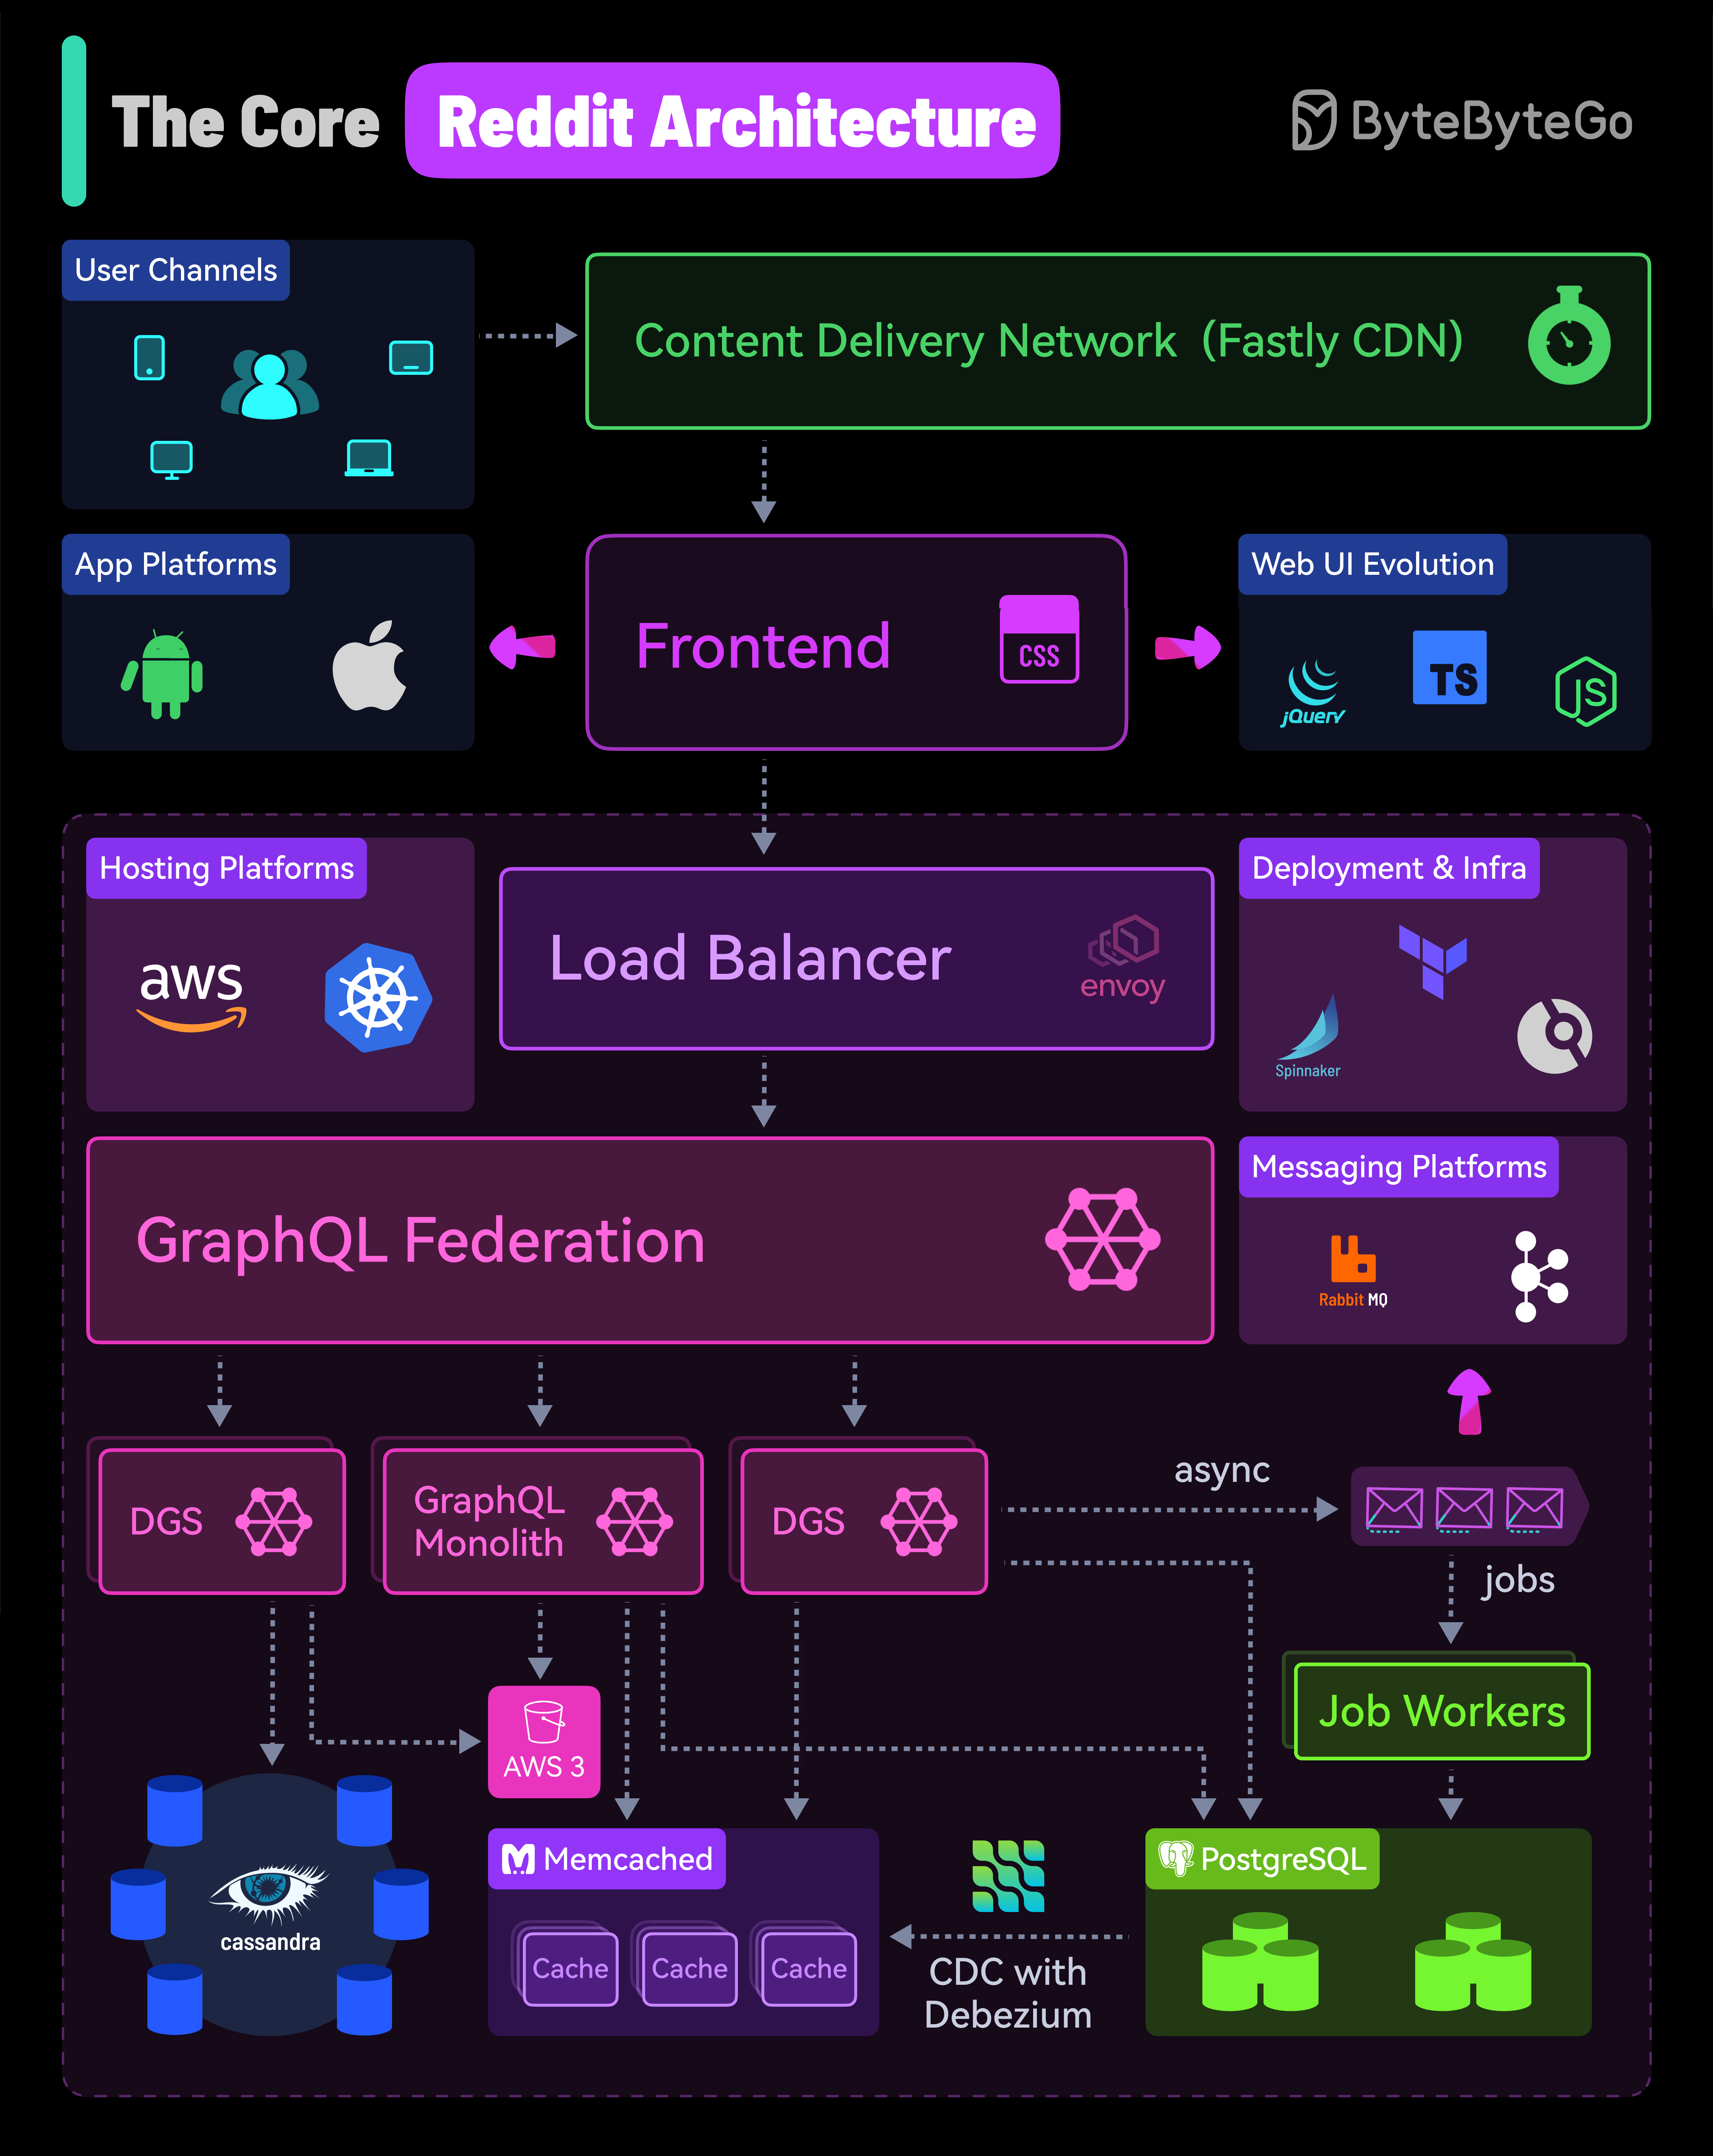
\includegraphics[width=\textwidth,height=.72\textheight,keepaspectratio]{img/0356-the-core-reddit-architecture.png}
    \caption{Reddit's core backend architecture \cite{bytebytego2024reddit}}
  \end{figure}
\end{frame}

%% ── Slide 6: Architecture Explained ──────────────────────────────────────────
\begin{frame}{Architecture: Solving the Three Goals}
  \begin{itemize}
    \item \structure{GraphQL Gateway} — single entry point (access transparency); routes requests to Go microservices
    \item \structure{Go Microservices} — each service scales independently (scalability); failures are isolated (fault tolerance)
    \item \structure{PostgreSQL (ThingDB)} — primary persistent store with read replicas (replication transparency)
    \item \structure{Memcached \& Redis} — multi-layer caching (efficiency); absorbs $>$95\% of read traffic before it hits the DB
    \item \structure{Kafka + Debezium (CDC)} — event streaming for eventual consistency; decouples producers from consumers
    \item \structure{RabbitMQ} — async background jobs (votes, emails); improves write throughput
    \item \structure{Cassandra} — high-availability NoSQL for time-series and voting data (fault tolerance across DCs)
    \item \structure{AWS / Kubernetes} — container orchestration and auto-scaling (scalability)
  \end{itemize}
  \vspace{1mm}
  {\footnotesize Source: \cite{bytebytego2024reddit}}
\end{frame}

%% ── Slide 7: Languages & API ──────────────────────────────────────────────────
\section{Technologies}
\begin{frame}{Languages \& API Layer}
  \begin{columns}[T]
    \begin{column}{.48\textwidth}
      \begin{block}{Python — Legacy Monolith (\texttt{r2})}
        \begin{itemize}
          \item Original language (2005)
          \item Handles routing and some business logic
          \item Bottleneck at scale → being phased out
        \end{itemize}
      \end{block}
      \vspace{2mm}
      \begin{block}{Go — Modern Microservices}
        \begin{itemize}
          \item Rewritten critical paths (comments, feeds)
          \item Goroutines: lightweight concurrency
          \item Significantly lower API latency
        \end{itemize}
      \end{block}
    \end{column}
    \begin{column}{.48\textwidth}
      \begin{block}{GraphQL Federation}
        \begin{itemize}
          \item Single unified API gateway for all clients (web, iOS, Android)
          \item Backend split into \textbf{Domain Graph Services (DGS)} subgraphs
          \item Teams deploy subgraphs independently → \alert{location transparency} for the client
          \item Prevents tight coupling between frontend and specific backend services
        \end{itemize}
      \end{block}
    \end{column}
  \end{columns}
  \vspace{1mm}
  {\footnotesize Source: \cite{stackshare2024reddit}, \cite{himalayas2024reddit}}
\end{frame}

%% ── Slide 8: Databases & Caching ─────────────────────────────────────────────
\begin{frame}{Databases \& Caching}
  \begin{columns}[T]
    \begin{column}{.48\textwidth}
      \begin{block}{PostgreSQL — ThingDB pattern}
        \begin{itemize}
          \item EAV (Entity-Attribute-Value) schema
          \item Stores posts, comments, accounts, votes
          \item Read replicas for \textbf{fault tolerance}
          \item Schema-less flexibility without migrations
        \end{itemize}
      \end{block}
      \vspace{2mm}
      \begin{block}{Redis}
      	\begin{itemize}
      		\item Structured cache + pub/sub broker
      		\item Stores leaderboards, rate limits, locks
      		%\item Acts as CDC event store (Change Data Capture)
      	\end{itemize}
      \end{block}
      
    \end{column}
    \begin{column}{.48\textwidth}
      \begin{block}{Apache Cassandra}
      	\begin{itemize}
      		\item Distributed, multi-datacenter NoSQL
      		\item Used for vote counts and time-series data
      		\item \alert{Tunable consistency} model (CAP trade-off)
      	\end{itemize}
      \end{block}
      \vspace{2mm}
      \begin{block}{Memcached}
      	\begin{itemize}
      		\item First caching layer in front of Postgres
      		\item Caches rendered posts, session tokens
      		\item Absorbs the majority of read traffic
      	\end{itemize}
      \end{block}
    \end{column}
  \end{columns}
  \vspace{1mm}
  {\footnotesize Source: \cite{bytebytego2024reddit}}
\end{frame}

%% ── Slide 9: Messaging & Infra ───────────────────────────────────────────────
\begin{frame}{Async Messaging \& Infrastructure}
  \begin{columns}[T]
    \begin{column}{.48\textwidth}
      \begin{block}{RabbitMQ — Background Jobs}
        \begin{itemize}
          \item AMQP queue for fire-and-forget tasks
          \item Votes, notifications, cleanups
          \item Decouples HTTP request cycle from heavy work
        \end{itemize}
      \end{block}
      \vspace{2mm}
      \begin{block}{Apache Kafka + Debezium (CDC)}
        \begin{itemize}
          \item Debezium tails PostgreSQL WAL logs
          \item Publishes change events to Kafka topics
          \item Consumers: search index, spam detection, analytics
          %\item Enables \textbf{eventual consistency} without tight coupling
        \end{itemize}
      \end{block}
    \end{column}
    \begin{column}{.48\textwidth}
      \begin{block}{AWS \& Kubernetes (EKS)}
        \begin{itemize}
          \item Multi-region AWS deployment
          \item Kubernetes auto-scales pods on traffic spikes
          \item \alert{Failure transparency}: crashed pods restart automatically
          \item ``Sister Datastore'' migration pattern: parallel writes to old \& new DB, compare results, then cut over safely
        \end{itemize}
      \end{block}
    \end{column}
  \end{columns}
  \vspace{1mm}
  {\footnotesize Source: \cite{bytebytego2024reddit}, \cite{himalayas2024reddit}}
\end{frame}

%% ── Slide 10: Bibliography ───────────────────────────────────────────────────
\section{\bibname}
\begin{frame}[t, allowframebreaks]{\bibname}
\printbibliography[heading=none]
\end{frame}

\end{document}
